\documentclass[tikz,border=10pt]{standalone}
\usepackage{tikz}
\usetikzlibrary{shapes.geometric, arrows.meta, positioning, fit, calc, shadows.blur, backgrounds}

% ==========================================
% Color Scheme
% ==========================================
\definecolor{cStep1}{RGB}{0, 105, 92}
\definecolor{cStep2}{RGB}{2, 119, 189}
\definecolor{cStep3}{RGB}{239, 108, 0}
\definecolor{cStep4}{RGB}{123, 31, 162}
\definecolor{bgGray}{RGB}{245, 245, 245}

\tikzset{
    mainBox/.style={
        rectangle, rounded corners=4pt,
        minimum width=5cm, minimum height=1.2cm,
        align=center, font=\bfseries\sffamily, text=white,
        blur shadow={shadow blur steps=5}
    },
    noteNode/.style={
        text width=4.5cm, align=left,
        font=\scriptsize\sffamily, color=gray!85!black
    },
    layerLabel/.style={
        font=\scriptsize\bfseries\sffamily,
        align=right, color=gray!60
    },
    flowArrow/.style={
        -{Latex[length=3mm, width=2mm]},
        line width=1.5pt, draw=gray!40
    }
}

\begin{document}
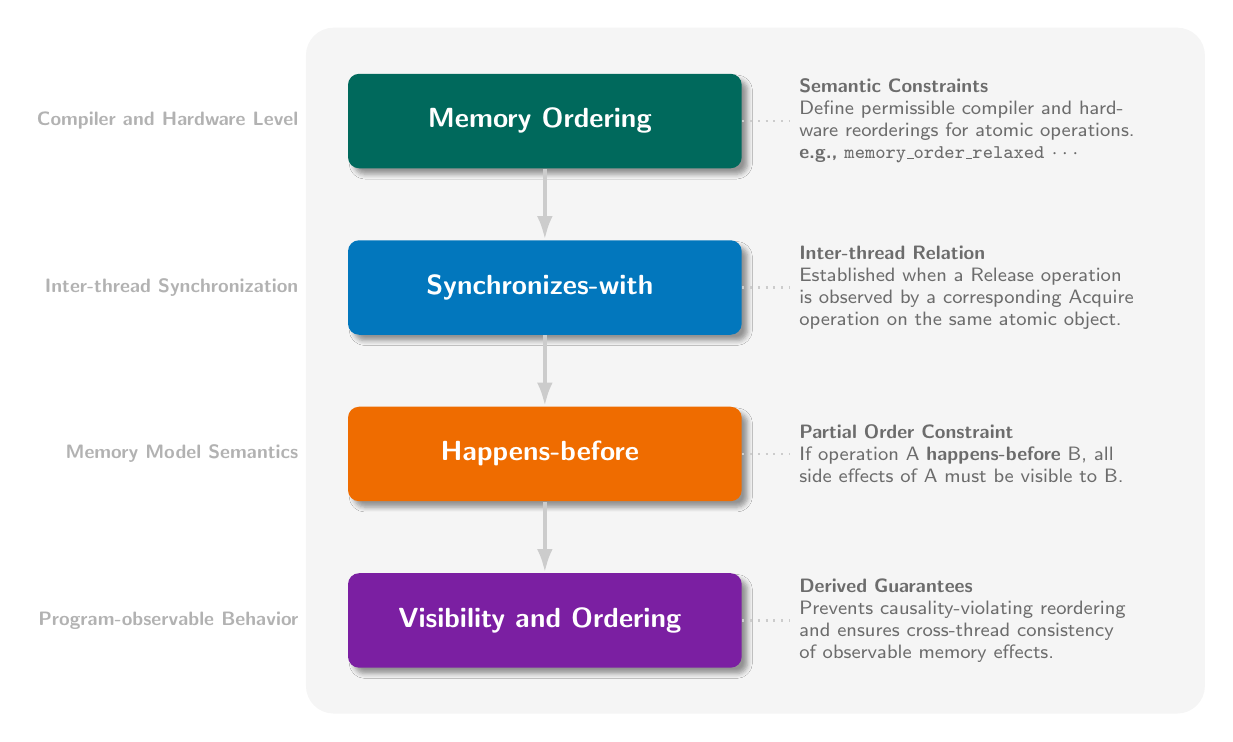
\begin{tikzpicture}[node distance=0.9cm]

	% =========================================================
	% Core Logical Flow
	% =========================================================

	\node [mainBox, fill=cStep1] (step1) {
		Memory Ordering
	};

	\node [mainBox, fill=cStep2, below=of step1] (step2) {
		Synchronizes-with
	};

	\node [mainBox, fill=cStep3, below=of step2] (step3) {
		Happens-before
	};

	\node [mainBox, fill=cStep4, below=of step3] (step4) {
		Visibility and Ordering
	};

	\draw [flowArrow] (step1) -- (step2);
	\draw [flowArrow] (step2) -- (step3);
	\draw [flowArrow] (step3) -- (step4);

	% =========================================================
	% Explanatory Notes
	% =========================================================

	\node [noteNode, right=0.6cm of step1] (note1) {
		\textbf{Semantic Constraints}\\
		Define permissible compiler and hardware reorderings for atomic operations.\\
		\textbf{e.g.,} \texttt{memory\_order\_relaxed} $\cdots$
	};

	\node [noteNode, right=0.6cm of step2] (note2) {
		\textbf{Inter-thread Relation}\\
		Established when a Release operation\\
		is observed by a corresponding Acquire\\
		operation on the same atomic object.
	};

	\node [noteNode, right=0.6cm of step3] (note3) {
		\textbf{Partial Order Constraint}\\
		If operation A \textbf{happens-before} B, all\\
		side effects of A must be visible to B.
	};

	\node [noteNode, right=0.6cm of step4] (note4) {
		\textbf{Derived Guarantees}\\
		Prevents causality-violating reordering\\
		and ensures cross-thread consistency\\
		of observable memory effects.
	};

	\foreach \i in {1,2,3,4} {
			\draw [dotted, thick, gray!40] (step\i.east) -- (note\i.west);
		}

	% =========================================================
	% Abstraction Layers
	% =========================================================

	\node [layerLabel, left=0.5cm of step1] {Compiler and Hardware Level};
	\node [layerLabel, left=0.5cm of step2] {Inter-thread Synchronization};
	\node [layerLabel, left=0.5cm of step3] {Memory Model Semantics};
	\node [layerLabel, left=0.5cm of step4] {Program-observable Behavior};

	% =========================================================
	% Background
	% =========================================================

	\begin{scope}[on background layer]
		\node [rectangle, fill=bgGray, rounded corners=10pt,
			fit=(step1)(step4)(note1)(note4), inner sep=15pt] {};
	\end{scope}

\end{tikzpicture}
\end{document}
